\documentclass[aspectratio=169,11pt]{beamer}

% ---------------------------------------------------------
% TP1 - BCC327 Computação Gráfica - UFOP 2026.2
% Baseado no template de apresentação CCO/DECOM
% ---------------------------------------------------------

% --- PACOTES PRINCIPAIS ---
\usepackage[utf8]{inputenc}
\usepackage[T1]{fontenc}
\usepackage[brazil]{babel}
\usepackage{amsmath, amssymb, amsfonts}
\usepackage{booktabs}
\usepackage{tabularx}
\usepackage{graphicx}
\usepackage{xcolor}
\usepackage{hyperref}
\usepackage{listings}
\usepackage{tikz}
\usetikzlibrary{arrows.meta, positioning}

\graphicspath{{figures/}}

% --- CORES INSTITUCIONAIS / ESTILO ---
\definecolor{ufopred}{RGB}{140,29,36}
\definecolor{deepnavy}{RGB}{20,35,60}
\definecolor{lightgray}{RGB}{245,247,250}
\definecolor{darkslate}{RGB}{30,40,50}
\definecolor{softblue}{RGB}{230,238,247}

% --- TEMA BEAMER ---
\usetheme{Madrid}
\usecolortheme{default}
\setbeamertemplate{navigation symbols}{}
\setbeamercolor{structure}{fg=ufopred}
\setbeamercolor{frametitle}{fg=white,bg=ufopred}
\setbeamercolor{title}{fg=white,bg=ufopred}
\setbeamercolor{block title}{fg=white,bg=deepnavy}
\setbeamercolor{block body}{fg=black,bg=lightgray}
\setbeamercolor{alerted text}{fg=ufopred}

% --- RODAPE PERSONALIZADO ---
\setbeamertemplate{footline}{%
  \leavevmode%
  \hbox{%
    \begin{beamercolorbox}[wd=.72\paperwidth,ht=2.6ex,dp=1.1ex,leftskip=1.5ex]{author in head/foot}%
      \usebeamerfont{author in head/foot}\textcolor{white}{\insertshorttitle}
    \end{beamercolorbox}%
    \begin{beamercolorbox}[wd=.28\paperwidth,ht=2.6ex,dp=1.1ex,rightskip=1.5ex plus1fil]{date in head/foot}%
      \usebeamerfont{date in head/foot}\hfill \textcolor{white}{\insertframenumber/\inserttotalframenumber}
    \end{beamercolorbox}%
  }%
}

% --- CONFIGURACAO DE CODIGO ---
\lstset{
  basicstyle=\ttfamily\small,
  keywordstyle=\color{ufopred}\bfseries,
  commentstyle=\color{darkslate},
  stringstyle=\color{deepnavy},
  showstringspaces=false,
  frame=single,
  rulecolor=\color{lightgray},
  breaklines=true
}

\newcommand{\checkitem}{\textcolor{ufopred}{$\blacktriangleright$}}

% ---------------------------------------------------------
% DADOS DA APRESENTACAO
% ---------------------------------------------------------
\title[TP1 -- Visualização, Rasterização e Recorte de Árvores CCO]{Visualização Geométrica, Rasterização e Recorte de Árvores Arteriais CCO}
\subtitle{Trabalho Prático 1 -- BCC327 Computação Gráfica}
\author{Heitor Augusto de Oliveira Ramos \and Rafael Stylita Duarte}
\institute[UFOP]{Departamento de Computação (DECOM)\\Universidade Federal de Ouro Preto (UFOP)}
\date{2026.2}

% ---------------------------------------------------------
\begin{document}

\begin{frame}
  \titlepage
\end{frame}

\begin{frame}{Roteiro da Apresentação}
\tableofcontents
\end{frame}

% =========================================================
\section{Contexto e Objetivos}
% =========================================================

\begin{frame}{Contexto do Trabalho}
\begin{block}{Problema}
Uma árvore CCO é só um conjunto de números: pontos, pares de índices e um raio por vaso. Para virar imagem, ela precisa passar por todas as etapas do \emph{pipeline} gráfico.
\end{block}

\vspace{0.25cm}

\begin{itemize}
  \item Modelos fornecidos em formato \texttt{.vtk} (ASCII, \texttt{POLYDATA}).
  \item Uma árvore 2D e uma 3D, ambas com 64 terminais.
  \item Cada vaso é um segmento entre dois pontos, com um atributo \texttt{raio}.
  \item Foco: entender e implementar os algoritmos clássicos, não só chamar a biblioteca.
\end{itemize}
\end{frame}

\begin{frame}{Objetivos}
\begin{block}{Objetivo Geral}
Uma aplicação única que lê, representa, transforma, rasteriza e recorta os modelos CCO, separando o que foi implementado pelo grupo do que vem da biblioteca.
\end{block}

\vspace{0.2cm}

\begin{columns}[T]
\column{0.5\textwidth}
\begin{itemize}
  \item[\checkitem] M1: leitura, primitivas e cor
  \item[\checkitem] M2: transformações, câmera e projeções
  \item[\checkitem] M3: Bresenham
  \item[\checkitem] M4: Scanline Fill
\end{itemize}
\column{0.5\textwidth}
\begin{itemize}
  \item[\checkitem] M5: aliasing e antialiasing
  \item[\checkitem] M6: Cohen--Sutherland e Liang--Barsky
  \item[\checkitem] M7: Sutherland--Hodgman
\end{itemize}
\end{columns}
\end{frame}

% =========================================================
\section{Dados e Metodologia}
% =========================================================

\begin{frame}{Dados Utilizados}
\begin{columns}
\column{0.48\textwidth}
\begin{itemize}
  \item \texttt{tree2D\_Nterm064.vtk} e \texttt{tree3D\_Nterm064.vtk}.
  \item Estrutura:
  \begin{itemize}
    \item \texttt{POINTS}: coordenadas $(x,y,z)$;
    \item \texttt{LINES}: \texttt{2 id\_início id\_fim};
    \item \texttt{CELL\_DATA}: escalar \texttt{raio} por segmento.
  \end{itemize}
  \item Leitor próprio, sem o leitor de VTK da biblioteca.
\end{itemize}

\column{0.48\textwidth}
\begin{block}{Modelos analisados}
\small
\begin{tabular}{lcc}
\toprule
 & \textbf{2D} & \textbf{3D}\\
\midrule
Pontos & 128 & 128\\
Segmentos & 127 & 127\\
Raio mínimo & 0,2032 & 0,2052\\
Raio máximo & 1,1814 & 1,0178\\
$r_{max}/r_{min}$ & 5,81 & 4,96\\
\bottomrule
\end{tabular}
\end{block}
\end{columns}
\end{frame}

\begin{frame}{Tecnologias Utilizadas}
\begin{itemize}
  \item Linguagem: Python 3.12.
  \item Biblioteca gráfica: PyVista 0.43.3 sobre VTK 9.3.0 (OpenGL).
  \item NumPy 1.26.4 para matrizes; Matplotlib 3.8.3 só para desenhar as figuras didáticas.
  \item Saída: visualizador interativo e figuras PNG para relatório e slides.
\end{itemize}

\vspace{0.25cm}

\begin{block}{Ambiente de execução}
\texttt{make install} cria o \texttt{venv} e instala as dependências fixadas; \texttt{make run-3d}, \texttt{make run-2d}, \texttt{make plots} e \texttt{make screenshots} executam a aplicação. O Makefile funciona em Linux/macOS e Windows.
\end{block}
\end{frame}

\begin{frame}{Fluxo Geral da Aplicação}
\begin{center}
\begin{tikzpicture}[node distance=0.5cm and 0.6cm,
  box/.style={draw=deepnavy, fill=lightgray, rounded corners, align=center, font=\small, minimum height=1.0cm, text width=2.7cm},
  own/.style={box, draw=ufopred, line width=1pt},
  arr/.style={-{Stealth}, thick, ufopred}]
\node[own] (vtk) {Leitura VTK\\\scriptsize\texttt{vtk\_loader.py}};
\node[box, right=of vtk] (model) {Geometria e atributos\\\scriptsize\texttt{CCOTreeModel}};
\node[own, right=of model, yshift=0.85cm] (view) {Transformações\\e câmera\\\scriptsize\texttt{viewer\_3d.py}};
\node[own, right=of model, yshift=-0.85cm] (cg) {Rasterização\\e recorte\\\scriptsize\texttt{rasterization.py}\\\scriptsize\texttt{clipping.py}};
\node[box, right=of view] (win) {Janela interativa\\(M1, M2, M5)};
\node[box, right=of cg] (fig) {Figuras didáticas\\(M3 a M7)};
\draw[arr] (vtk) -- (model);
\draw[arr] (model) -- (view);
\draw[arr] (model) -- (cg);
\draw[arr] (view) -- (win);
\draw[arr] (cg) -- (fig);
\end{tikzpicture}
\end{center}
\vspace{0.2cm}
\small Borda vermelha: algoritmos implementados pelo grupo. Um único \texttt{main.py} com três modos: \texttt{viewer}, \texttt{plots} e \texttt{screenshots}.
\end{frame}

% =========================================================
\section{Implementação}
% =========================================================

\begin{frame}{Representação Geométrica e Cores}
\begin{columns}[T]
\column{0.40\textwidth}
\small
\begin{itemize}
  \item Cada vaso é um \textbf{tubo próprio}, com 2 pontos exclusivos: o raio não é interpolado entre vasos vizinhos.
  \item Espessura $\propto$ raio do arquivo.
  \item Mapa contínuo \texttt{coolwarm} (azul = fino, vermelho = grosso): o raio é contínuo, e uma paleta RGB discreta criaria fronteiras artificiais.
  \item Tecla \texttt{C}: espessura constante, só a cor codifica o raio.
\end{itemize}
\column{0.58\textwidth}
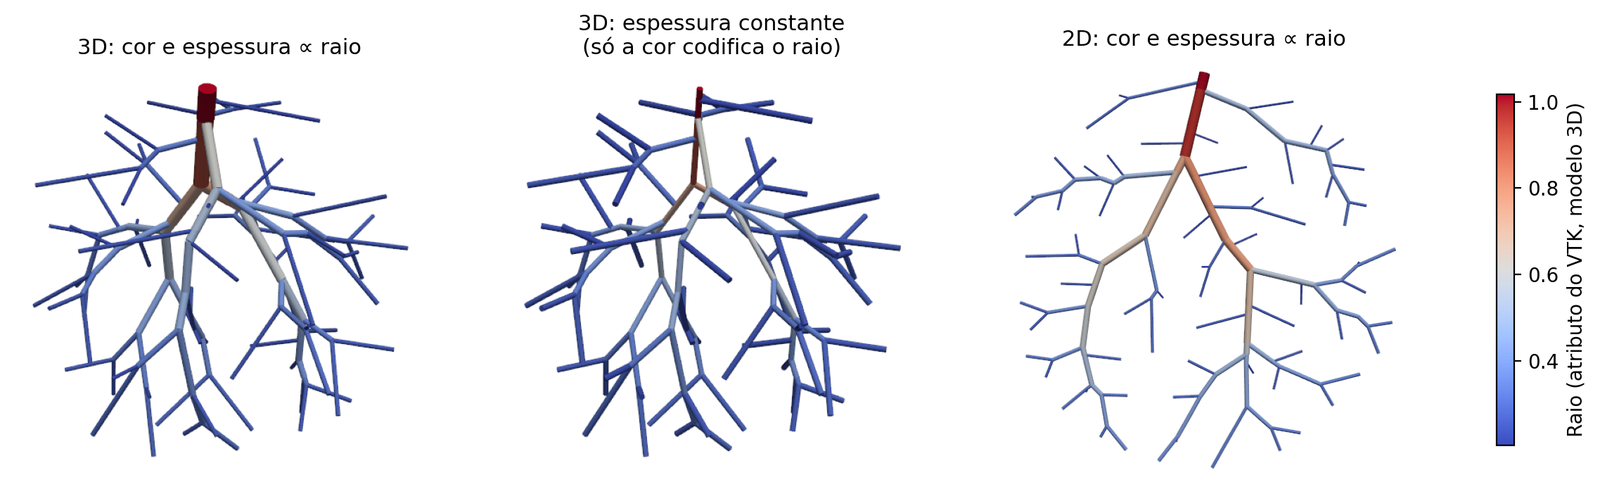
\includegraphics[width=\textwidth]{mod1_primitivas.png}
\end{columns}
\end{frame}

\begin{frame}{Transformações Geométricas}
\begin{center}
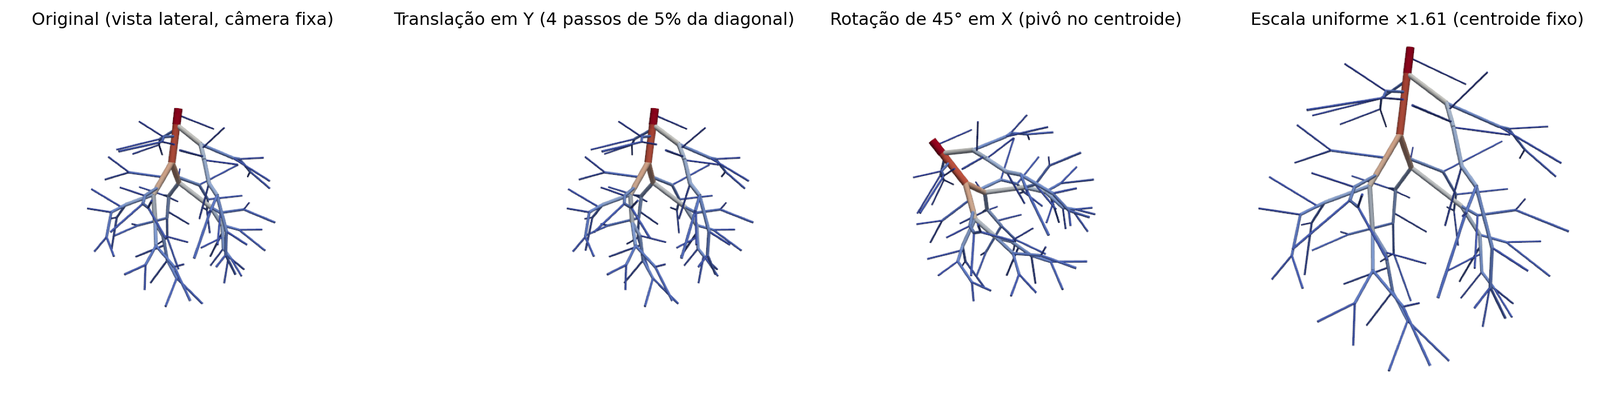
\includegraphics[width=0.9\textwidth]{mod2_transformacoes.png}
\end{center}
\vspace{-0.3cm}
\begin{columns}[T]
\column{0.48\textwidth}
\footnotesize
\begin{itemize}
  \item Matrizes homogêneas $4\times4$ em NumPy: $T(\mathbf{d})$, $R_x, R_y, R_z(\theta)$, $S(s)$.
  \item Em torno do centroide: $M' = T(\mathbf{c})\, M\, T(-\mathbf{c})$.
  \item Acúmulo $M_{acc} \leftarrow M'\,M_{acc}$, impresso no terminal.
\end{itemize}
\column{0.48\textwidth}
\footnotesize
\begin{itemize}
  \item Teclas: \texttt{T/G} translação, \texttt{K/J} rotação de $15^\circ$, \texttt{+/-} escala, \texttt{0} reinicia.
  \item Câmera fixa: a mudança na imagem vem só das coordenadas no mundo.
\end{itemize}
\end{columns}
\end{frame}

\begin{frame}{Câmera, Vistas e Projeções}
\begin{columns}[T]
\column{0.40\textwidth}
\small
\begin{itemize}
  \item \textbf{Mundo}: coordenadas do modelo após as transformações.
  \item \textbf{Câmera}: base $(\mathbf{u},\mathbf{v},\mathbf{w})$ a partir de posição, foco e \emph{up}; o observador fica na origem.
  \item Vistas: \texttt{B} frontal, \texttt{N} lateral, \texttt{U} superior, \texttt{I} isométrica.
  \item \texttt{O} ortográfica: tamanho não depende da profundidade.
  \item \texttt{V} perspectiva: $x_p = d\,x_c/(-z_c)$.
\end{itemize}
\column{0.58\textwidth}
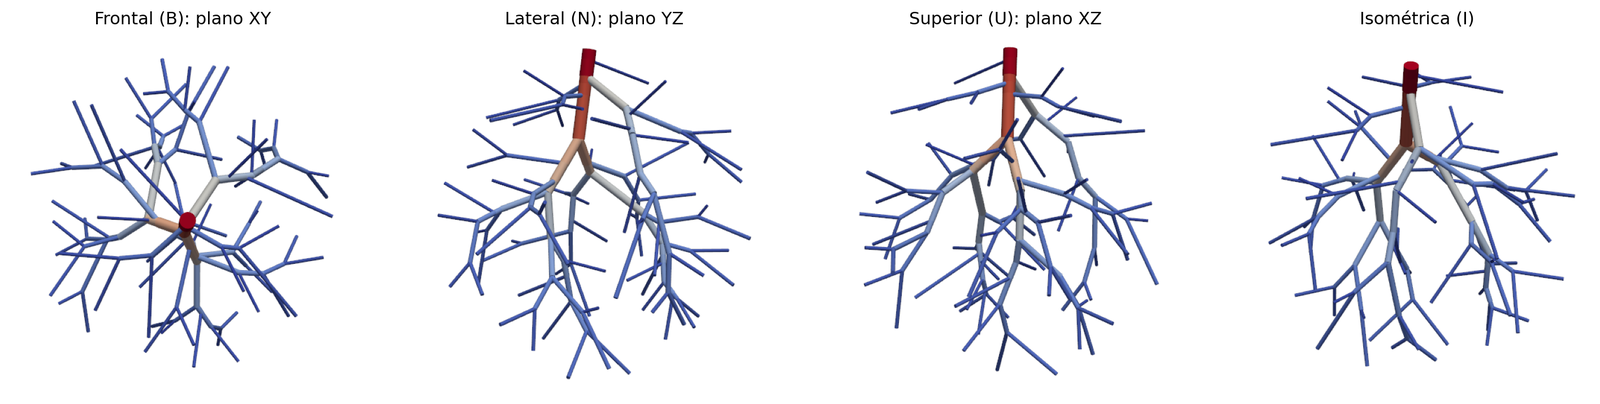
\includegraphics[width=\textwidth]{mod2_vistas.png}

\vspace{0.15cm}
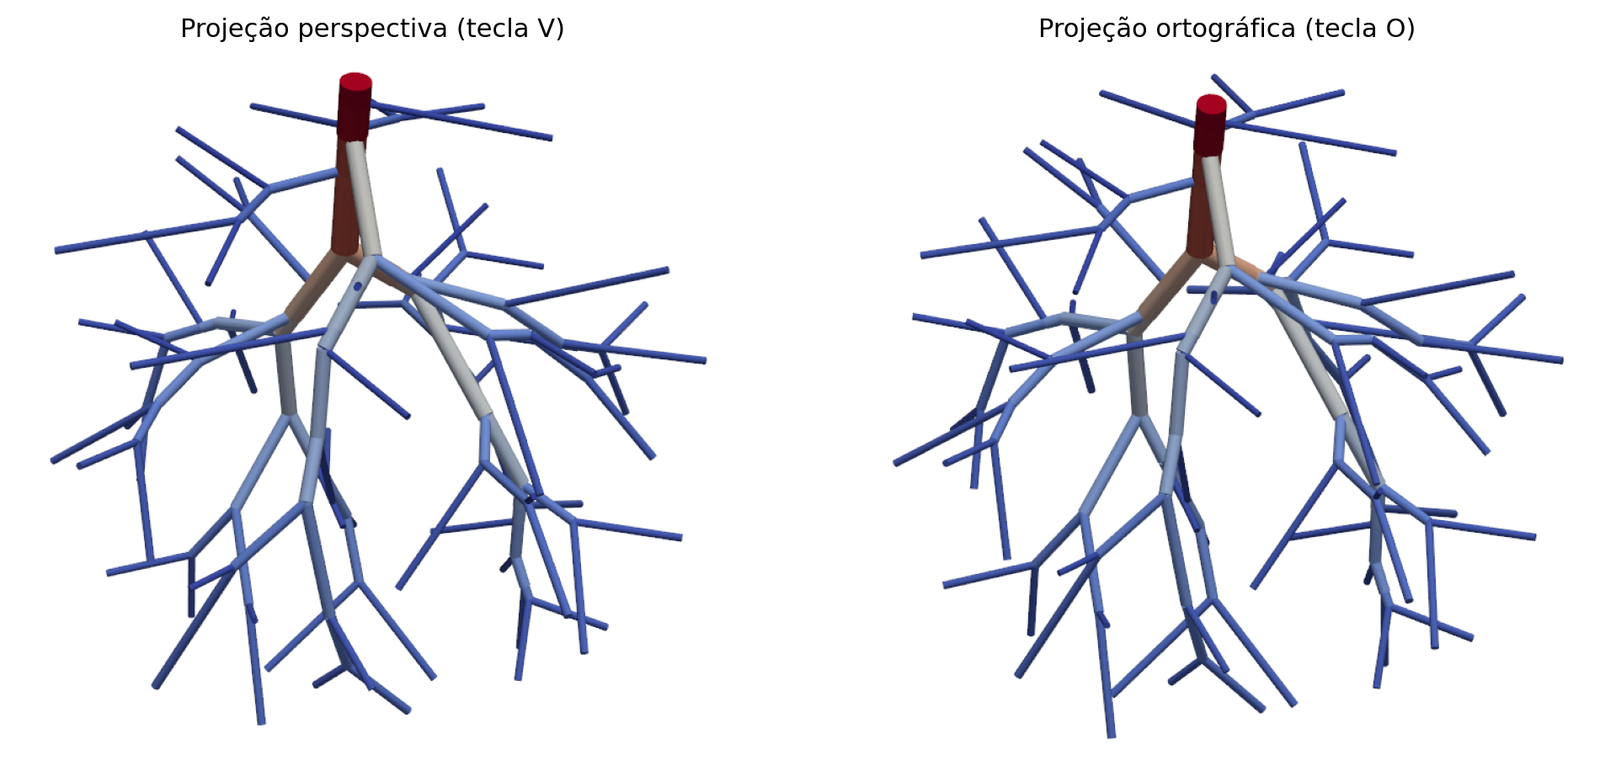
\includegraphics[width=0.85\textwidth]{mod2_projecoes.png}
\end{columns}
\end{frame}

\begin{frame}{Técnicas de Computação Gráfica Implementadas}
\small
\begin{tabularx}{\textwidth}{p{0.27\textwidth} X p{0.17\textwidth}}
\toprule
\textbf{Técnica} & \textbf{Como foi utilizada no projeto} & \textbf{Origem}\\
\midrule
Transformações & matrizes $4\times4$ de translação, rotação e escala com pivô & grupo\\
Câmera / projeções & 4 vistas; ortográfica $\times$ perspectiva & PyVista\\
Rasterização de linhas & Bresenham nos 8 octantes, aritmética inteira & grupo\\
Rasterização de polígonos & Scanline Fill com ET e AET, regra par-ímpar & grupo\\
Antialiasing & supersampling $k\times k$ por cobertura; MSAA/SSAA no viewer & grupo / VTK\\
Recorte de segmentos & Cohen--Sutherland e Liang--Barsky (Cyrus--Beck discutido) & grupo\\
Recorte de polígonos & Sutherland--Hodgman (Weiler--Atherton discutido) & grupo\\
\bottomrule
\end{tabularx}
\end{frame}

% =========================================================
\section{Resultados}
% =========================================================

\begin{frame}{Módulo 3: Bresenham}
\begin{columns}[T]
\column{0.36\textwidth}
\small
\begin{itemize}
  \item $(2,3)\to(14,10)$: $\Delta x=12$, $\Delta y=7$.
  \item $e = \Delta x-\Delta y = 5$; a cada passo $e_2=2e$:
  \begin{itemize}
    \item $e_2 > -\Delta y$: avança $x$;
    \item $e_2 < \Delta x$: avança $y$.
  \end{itemize}
  \item $\max(12,7)+1 = 13$ pixels, só com somas inteiras.
  \item À direita: os 127 vasos da árvore 2D numa grade $60\times60$.
\end{itemize}
\column{0.62\textwidth}
\vspace{0.2cm}
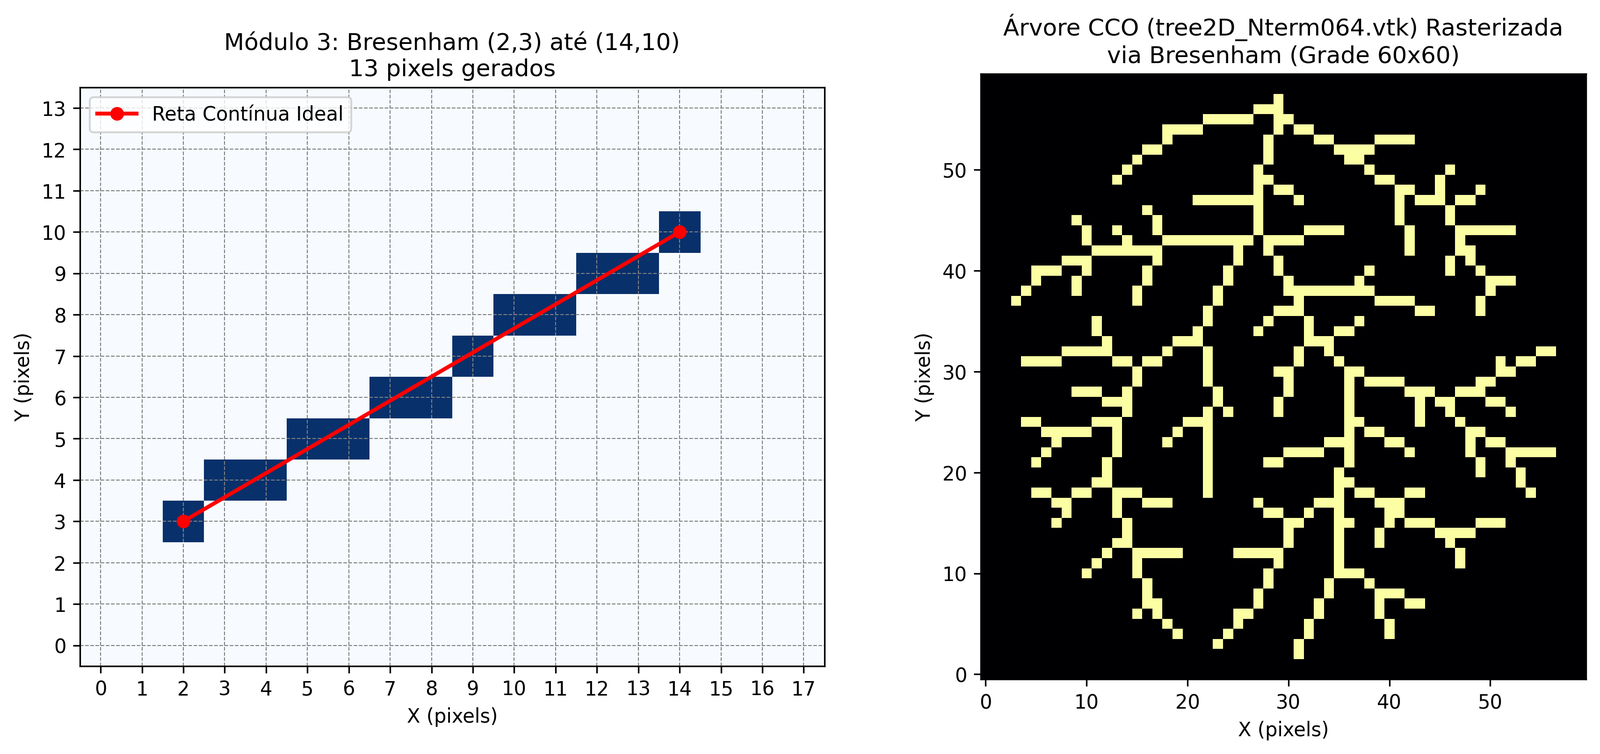
\includegraphics[width=\textwidth]{mod3_bresenham.png}
\end{columns}
\end{frame}

\begin{frame}{Módulo 4: Scanline Fill}
\begin{center}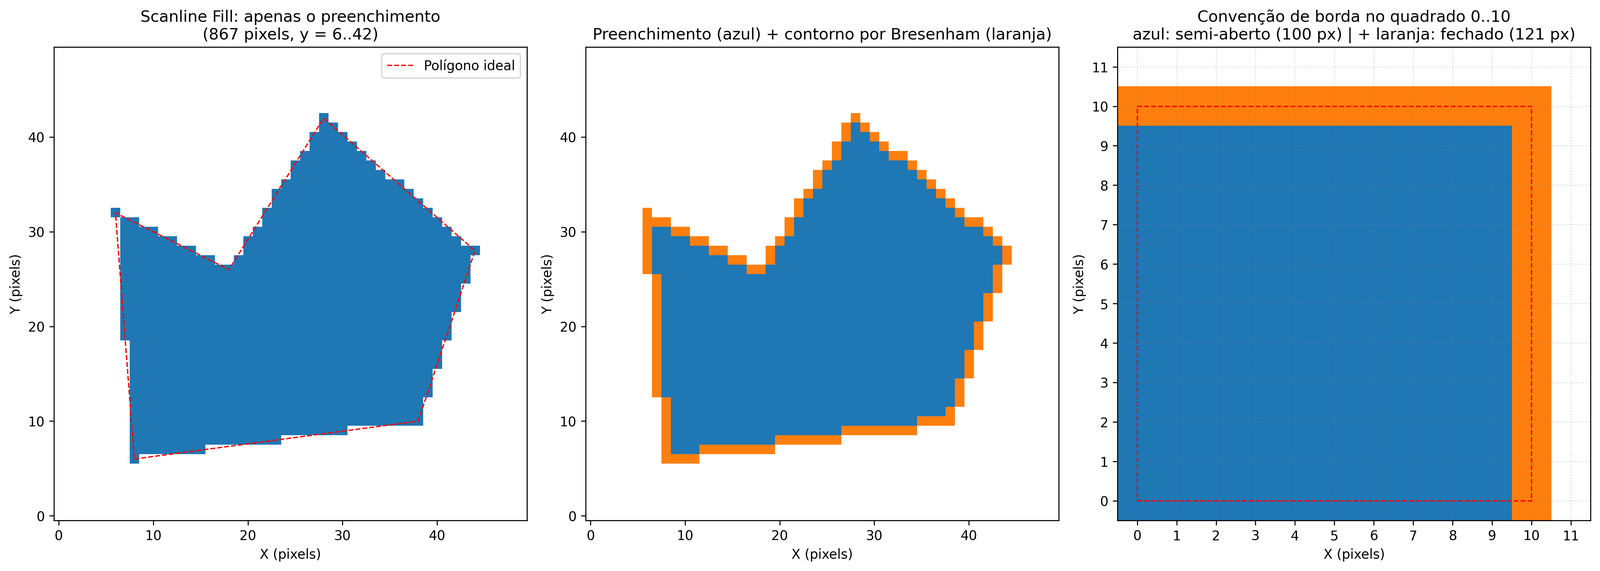
\includegraphics[width=0.88\textwidth]{mod4_scanline.png}\end{center}

\vspace{0.1cm}
\small
\begin{itemize}
  \item Polígono côncavo de 6 vértices: 867 pixels nas linhas $y=6..42$.
  \item Arestas ativas em $[y_{min}, y_{max})$: vértices compartilhados não são contados duas vezes.
  \item Quadrado $0..10$: 121 pixels (fechado) $\times$ 100 pixels (semiaberto, sem sobreposição entre vizinhos).
\end{itemize}
\end{frame}

\begin{frame}{Módulo 5: Aliasing $\times$ Antialiasing}
\begin{columns}[T]
\column{0.57\textwidth}
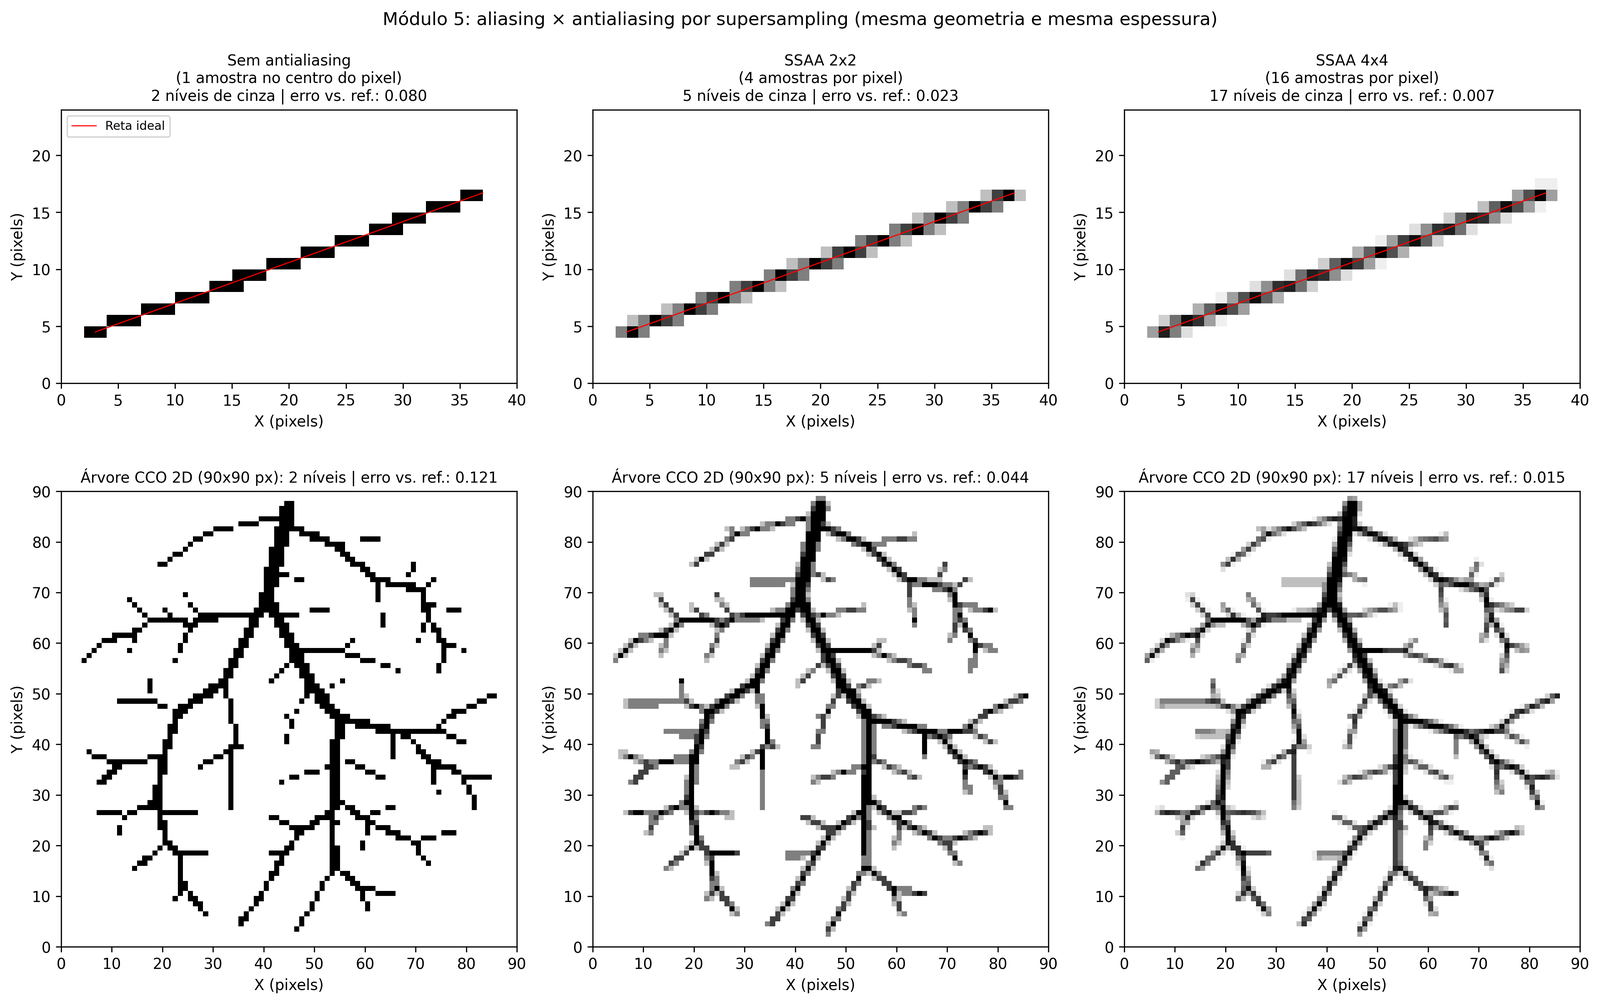
\includegraphics[width=\textwidth]{mod5_antialiasing.png}
\column{0.41\textwidth}
\footnotesize
\setlength{\tabcolsep}{3pt}
Mesma geometria e espessura; só muda o número de amostras por pixel.

\vspace{0.15cm}
\begin{tabular}{lccc}
\toprule
\textbf{Amostras} & \textbf{Níveis} & \textbf{Erro reta} & \textbf{Erro árvore}\\
\midrule
1 & 2 & 0,080 & 0,121\\
$2\times2$ & 5 & 0,023 & 0,044\\
$4\times4$ & 17 & 0,007 & 0,015\\
\bottomrule
\end{tabular}

\vspace{0.2cm}
\begin{itemize}
  \item Sem AA: escada na reta e vasos finos fragmentados.
  \item $4\times4$: erro $\approx 11\times$ menor, custo $16\times$ maior.
\end{itemize}
\end{columns}
\end{frame}

\begin{frame}{Módulo 5: Antialiasing no Visualizador}
\begin{center}
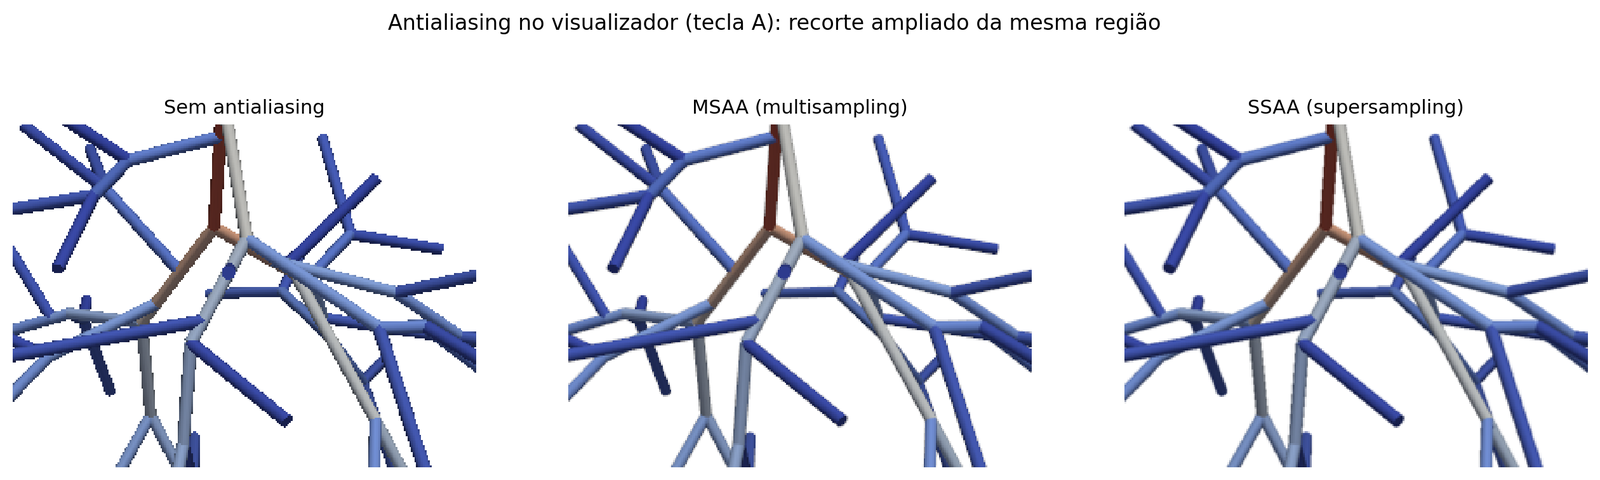
\includegraphics[width=0.95\textwidth]{mod5_viewer_aa.png}
\end{center}
\small
\begin{itemize}
  \item Tecla \texttt{A}: desligado $\to$ MSAA $\to$ SSAA (fornecidos pelo VTK).
  \item MSAA: várias amostras de cobertura por pixel, cor calculada uma vez por primitiva.
  \item SSAA: renderiza em resolução maior e reduz, mais caro e trata também o sombreamento.
\end{itemize}
\end{frame}

\begin{frame}{Módulo 6: Recorte de Segmentos}
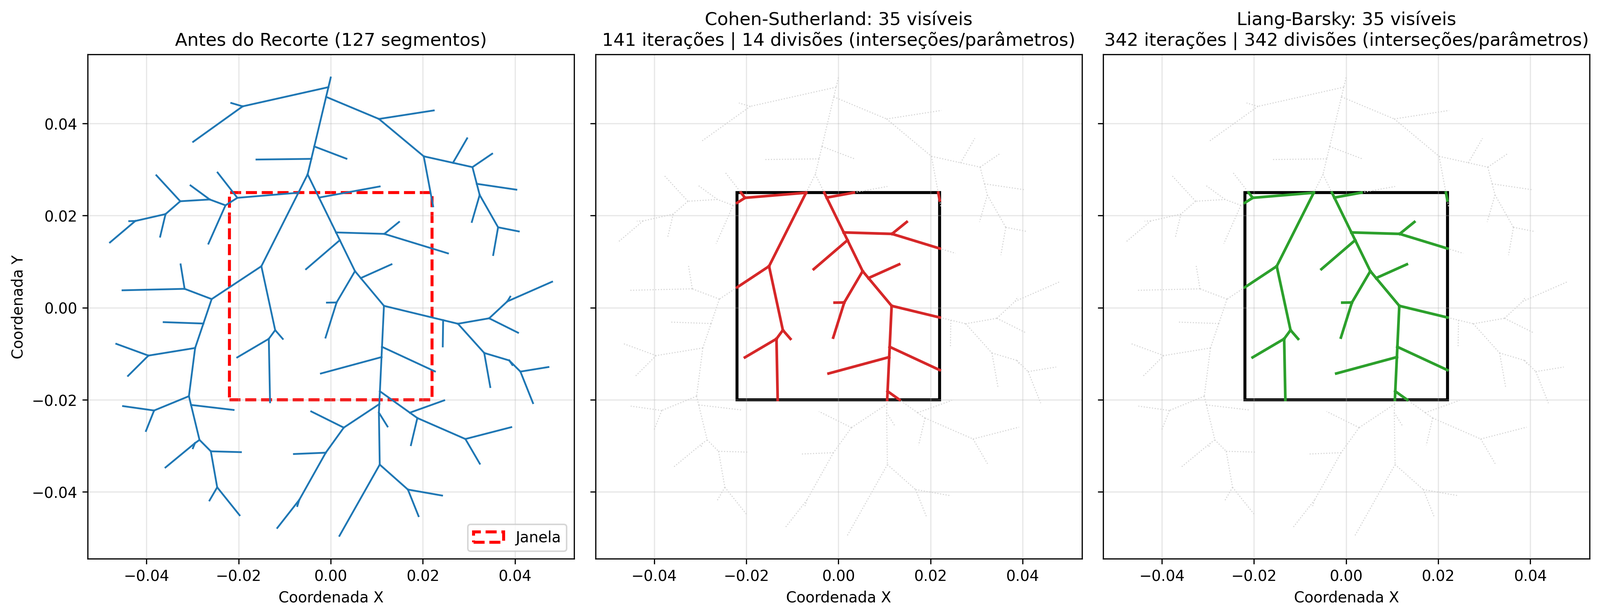
\includegraphics[width=\textwidth]{mod6_line_clipping.png}

\small
Janela $[-0{,}022;\,0{,}022]\times[-0{,}020;\,0{,}025]$: \textbf{35 segmentos visíveis nos dois algoritmos, 0 divergências}.
\end{frame}

\begin{frame}{Módulo 6: Comparação de Custo}
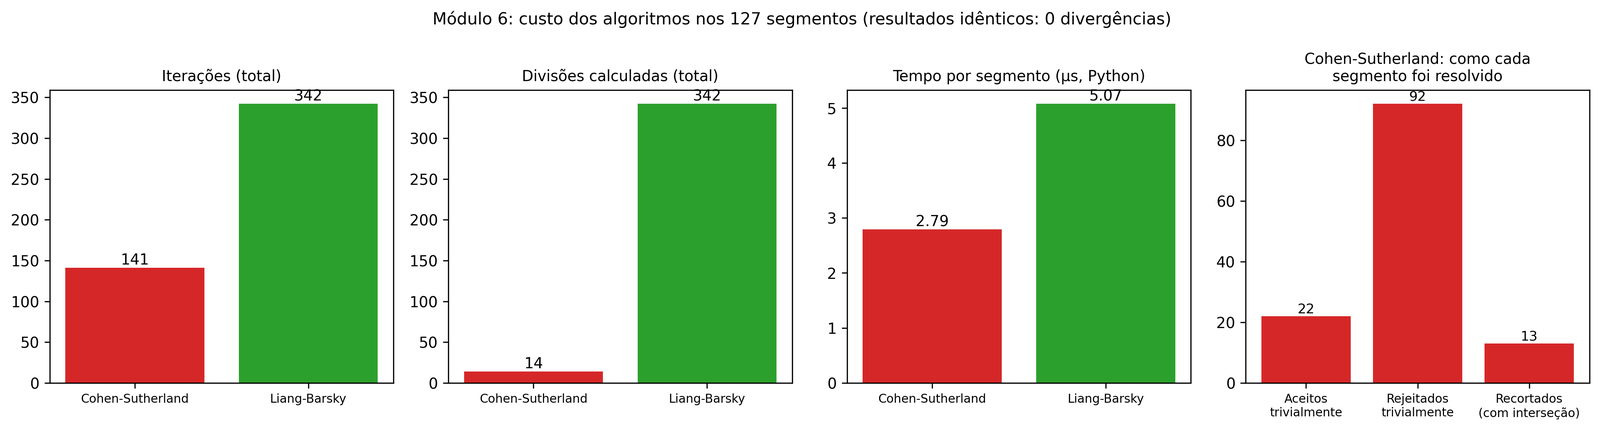
\includegraphics[width=\textwidth]{mod6_comparacao_algoritmos.png}

\vspace{0.1cm}
\small
\begin{itemize}
  \item \textbf{Cohen--Sutherland}: 114 de 127 segmentos resolvidos só com códigos de região; 14 interseções.
  \item \textbf{Liang--Barsky}: sempre 4 testes de borda (342 divisões), mas calcula cada extremo uma única vez. Vantajoso quando muitos segmentos cruzam a janela.
  \item \textbf{Cyrus--Beck}: mesma ideia paramétrica para janelas \emph{convexas quaisquer}, usando normais $\mathbf{N}_i$; Liang--Barsky é o caso retangular.
\end{itemize}
\end{frame}

\begin{frame}{Módulo 7: Recorte de Polígonos}
\begin{columns}[T]
\column{0.42\textwidth}
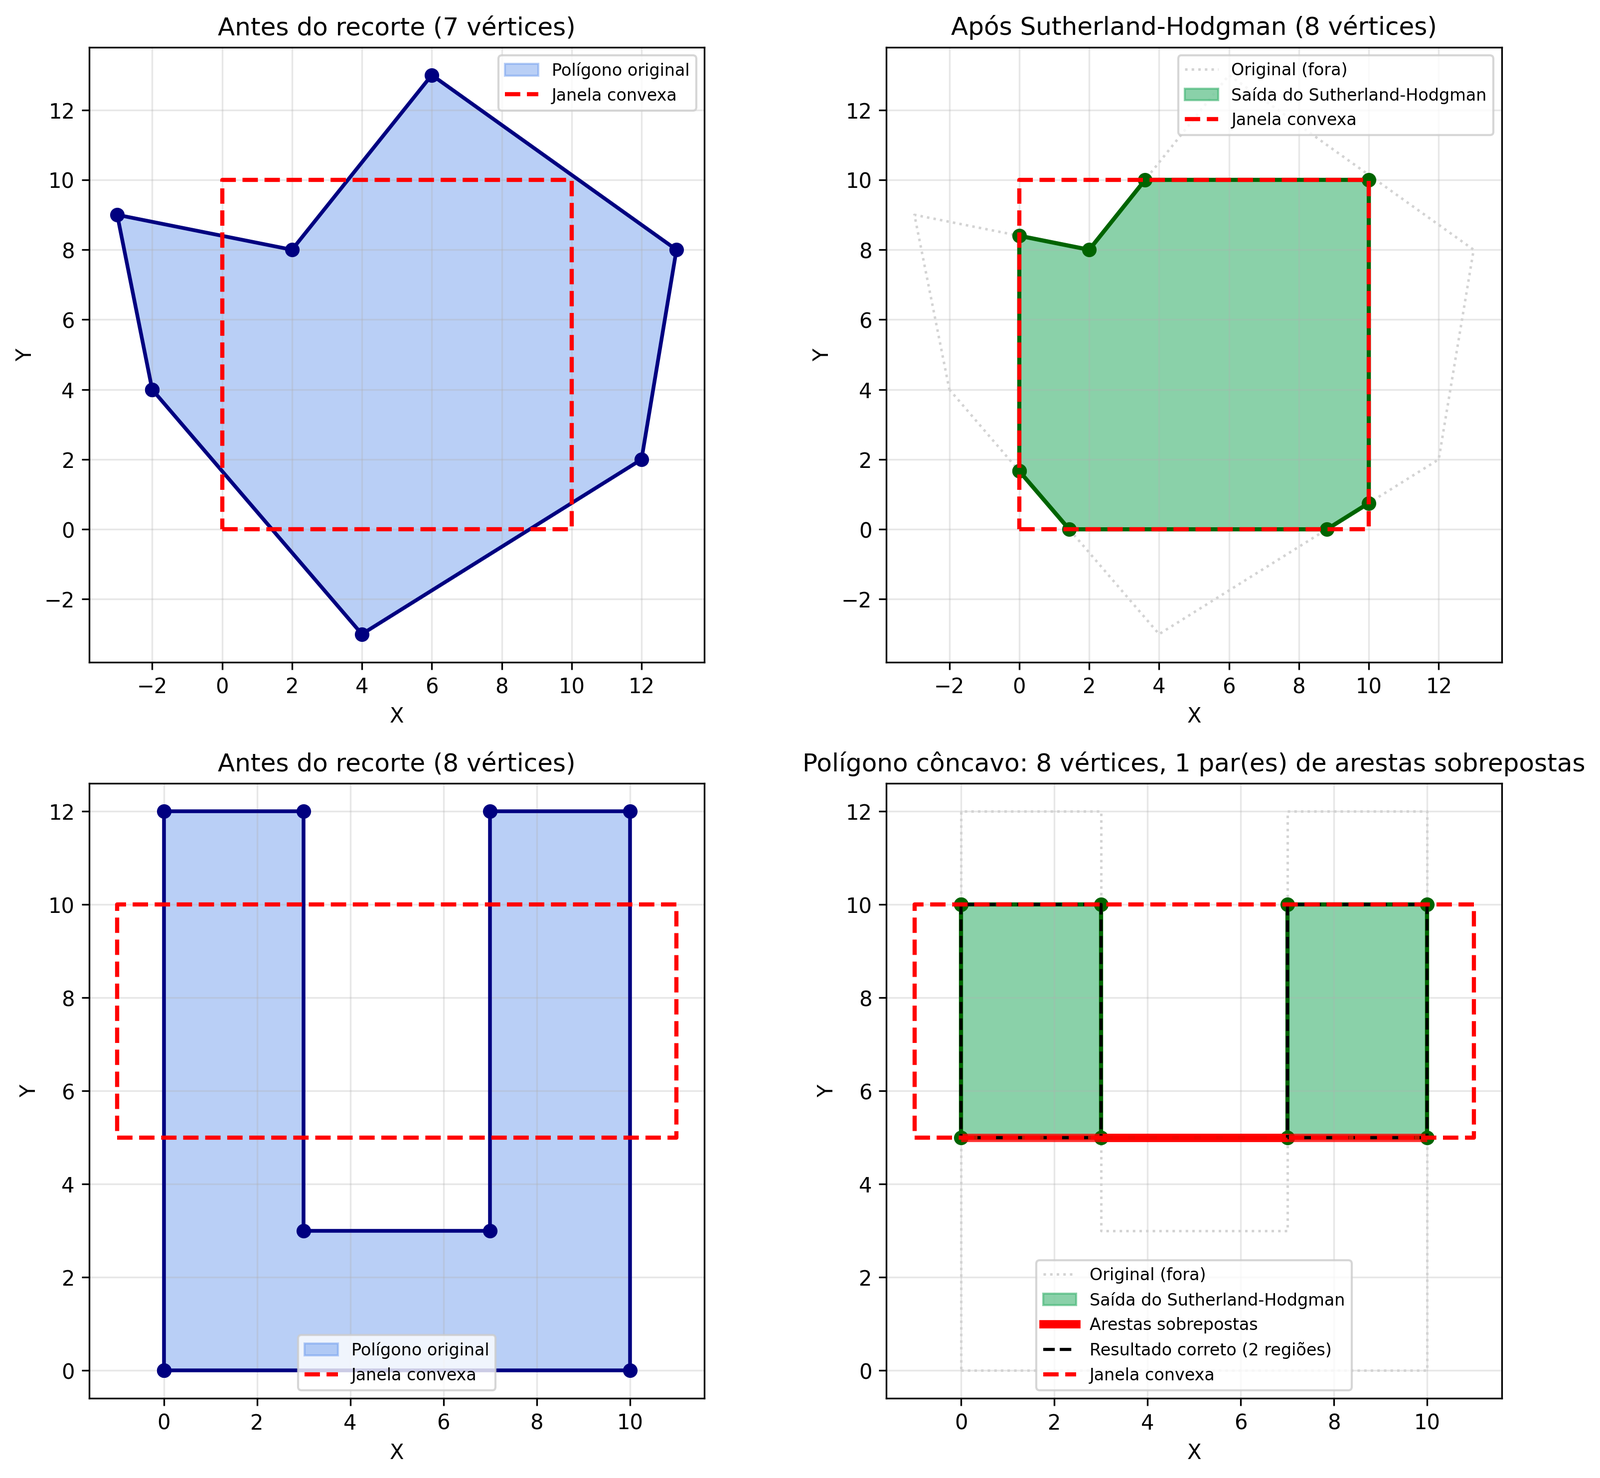
\includegraphics[width=\textwidth]{mod7_polygon_clipping.png}
\column{0.56\textwidth}
\footnotesize
\begin{block}{Sutherland--Hodgman}
Recorta contra cada aresta da janela convexa (4 casos dentro/fora). Janela validada e reorientada para anti-horário.
\end{block}
\begin{itemize}
  \item Caso 1: 7 vértices $\to$ 8 vértices, resultado correto.
  \item Caso ``U'': o correto são 2 regiões, mas a saída é 1 lista de 8 vértices com \textbf{arestas sobrepostas} em $y=5$.
\end{itemize}
\begin{block}{Quando usar Weiler--Atherton}
Polígonos côncavos que se dividem em várias regiões, janelas côncavas, buracos e operações booleanas: percorre as fronteiras alternando nas interseções e devolve várias regiões.
\end{block}
\end{columns}
\end{frame}

\begin{frame}{Recurso Adicional}
\begin{block}{Medição e reprodutibilidade dos resultados}
Os algoritmos de recorte contam iterações, divisões e casos triviais (\texttt{ClipStats}); o antialiasing mede níveis de cinza e erro contra uma referência $16\times16$; o modo \texttt{screenshots} regera as capturas do visualizador sem abrir janela.
\end{block}

\begin{itemize}
  \item \textbf{Motivação:} comparar algoritmos com números, e não só visualmente.
  \item \textbf{Como:} contadores opcionais nas funções de recorte; \texttt{CCOViewer} em modo \emph{off-screen} acionado pelos mesmos métodos das teclas.
  \item \textbf{Resultado:} todas as figuras e tabelas do relatório são regeradas com \texttt{make plots} e \texttt{make screenshots}.
\end{itemize}
\end{frame}

% =========================================================
\section{Discussão e Conclusão}
% =========================================================

\begin{frame}{Discussão}
\begin{columns}[T]
\column{0.5\textwidth}
\small
\begin{block}{Implementado pelo grupo}
Leitor VTK; matrizes $4\times4$ e pivô; tubos por segmento; Bresenham; Scanline (ET/AET); supersampling; Cohen--Sutherland; Liang--Barsky; Sutherland--Hodgman.
\end{block}
\begin{block}{Com auxílio de biblioteca}
PyVista/VTK: janela, câmera, projeções, malha dos tubos, mapa de cores, iluminação, MSAA/SSAA. Matplotlib: só exibição.
\end{block}
\column{0.48\textwidth}
\small
\begin{itemize}
  \item \textbf{Dificuldades:} raio interpolado entre vasos (resolvido com pontos duplicados); vértices compartilhados no Scanline; comparação justa de antialiasing.
  \item \textbf{Limitações:} recorte e rasterização didáticos no plano $XY$; malha reconstruída a cada transformação; Weiler--Atherton e Cyrus--Beck só discutidos.
  \item \textbf{Melhorias:} matriz aplicada na GPU, esferas nas bifurcações, Weiler--Atherton.
\end{itemize}
\end{columns}
\end{frame}

\begin{frame}{Conclusões}
\begin{itemize}
  \item Os sete módulos do TP1 foram atendidos sobre os modelos CCO 2D e 3D.
  \item Supersampling $4\times4$ reduziu o erro de cobertura em cerca de 11 vezes.
  \item Cohen--Sutherland e Liang--Barsky: mesmo recorte, custos diferentes conforme a cena.
  \item O caso côncavo mostra na prática a limitação do Sutherland--Hodgman.
  \item Base pronta para o TP2: Z-buffer, iluminação, transparência e \emph{ray casting}.
\end{itemize}

\vspace{0.25cm}

\begin{block}{Mensagem final}
Cada pixel da árvore CCO na tela passou por algoritmos que o grupo implementou ou consegue explicar, da leitura do VTK ao recorte.
\end{block}
\end{frame}

\begin{frame}{Referências}
\small
\begin{thebibliography}{99}
\bibitem{foley} FOLEY, J. D. et al. \textit{Computer Graphics: Principles and Practice}. Addison-Wesley, 1996.
\bibitem{hearn} HEARN, D.; BAKER, M. \textit{Computer Graphics with OpenGL}. Pearson, 2011.
\bibitem{angel} ANGEL, E.; SHREINER, D. \textit{Interactive Computer Graphics}. Pearson, 2015.
\bibitem{schreiner1993} SCHREINER, W.; BUXBAUM, P. Computer-optimization of vascular trees. \textit{IEEE Transactions on Biomedical Engineering}, 1993.
\bibitem{liang} LIANG, Y.-D.; BARSKY, B. A. A new concept and method for line clipping. \textit{ACM TOG}, 1984.
\bibitem{sh} SUTHERLAND, I. E.; HODGMAN, G. W. Reentrant polygon clipping. \textit{CACM}, 1974.
\bibitem{vtk} VTK Documentation. \url{https://vtk.org/} \quad PyVista. \url{https://docs.pyvista.org/}
\end{thebibliography}
\end{frame}

% ---------------------------------------------------------
\appendix
\section{Apêndice}

\begin{frame}[fragile]{Comandos de Execução}
\begin{lstlisting}[language=bash]
make install          # cria o venv e instala as dependencias
make run-3d           # visualizador interativo, modelo 3D
make run-2d           # visualizador interativo, modelo 2D
make plots            # figuras dos modulos 3 a 7
make screenshots      # capturas do visualizador (modulos 1, 2 e 5)
make clean            # remove venv e __pycache__
\end{lstlisting}

\begin{block}{Observação}
O README traz dependências e versões, teclas do visualizador e um roteiro mínimo de teste.
\end{block}
\end{frame}

\begin{frame}{Obrigado!}
\begin{center}
{\Huge Obrigado!}\\[0.5cm]
{\large Perguntas?}\\[0.5cm]
Heitor Augusto de Oliveira Ramos \quad\textbullet\quad Rafael Stylita Duarte
\end{center}
\end{frame}

\end{document}
